
\section{Compression}
\label{sec:compression}

This section describes \name's compressed representation, selected new concepts, and the overall compression algorithm.
The new encoding schemes are designed for redundancy exploitation across operations, while the new compression algorithm ensures fast, easy to amortize compression.

\subsection{Compressed Representation}
\label{sec:compressedRepresentation}


\begin{table}[!t]
    \centering \setlength\tabcolsep{10pt}
    \caption{\label{tab:colgroups}Overview of CLA and \name \ Column Groups.}
    \vspace{-0.4cm}
    \begin{tabular}{llcc}
        \toprule
        \textbf{Type} & \textbf{Description}      & \textbf{CLA}~\cite{ElgoharyBHRR16,ElgoharyBHRR18} & \textbf{\name} \\
        \midrule
        CON           & Constant or Empty Columns &                                                   & \checkmark     \\
        DDC           & Dense Dictionary Coding   & \checkmark                                        & \checkmark     \\
        OLE           & Offset-list Encoding      & \checkmark                                        & (\checkmark)   \\
        FOR           & Frame of Reference        &                                                   & \checkmark     \\
        RLE           & Run-length Encoding       & \checkmark                                        & (\checkmark)   \\
        SDC           & Sparse Dictionary Coding  &                                                   & \checkmark     \\
        UC            & Uncompressed (dense/sparse) & \checkmark                                        & \checkmark     \\
        \bottomrule
    \end{tabular}
    \vspace{0.1cm}
\end{table}


% with the ``best'' encoding type, by some objective.
% Our optimizers minimize compression size, workload cost or hybrid costs combining multiple objectives.

\name\ encodes each column group independently in a specific encoding type.
Table~\ref{tab:colgroups} shows these column-group encodings, as well as the differences to CLA.
Figure~\ref{fig:encoded} then presents an example of compressing a $10\times 6$ matrix into three single-column groups (0, 2 and 5), one two-column group ($\{1,3\}$), and an empty group. Also shown is an element-wise scalar subtraction on the compressed matrix, creating two alternative compressed outputs (A and B).


\textbf{Dense Dictionary Coding (DDC)} contains two parts: a \emph{dictionary} with the distinct value tuples in the column group,
(shown in Figure~\ref{fig:encoded} as a Dict with 2 values for column $\{0\}$), and an \emph{index structure} with a row-to-tuple mapping (e.g., dictionary position). DDC is dense because each row input is assigned a code in the map.

\textbf{Sparse Dictionary Coding (SDC)}
is a combination of DDC and sparse matrix formats like compressed sparse rows (CSR).
An example is shown in yellow for columns $\{1,3\}$ in Figure~\ref{fig:encoded}. Like DDC, each group has a dictionary of all unique tuples except the most frequent tuple named ``Def'' for default. This scheme encodes row locations of non-default tuples in the index structure as row-index pairs. This approach is similar to compressed sparse columns (CSC) that store row-index/value pairs for non-zero values, but extends it for general redundancy exploitation (default values, dictionary references).
% SDC Index structure
The row part is further specialized to delta offsets (``Off'') from previous rows to allow smaller physical codewords.
Finally, a ``Map'' (index part of CSC) maps offsets to tuples in the dictionary, similar to DDC.
% Specialization
SDC specializes into SDCZero, where zero default entries are removed like in the
$\{2\}$
blue column group, and SDCSingle for binary data (one dictionary entry, one default), removing the need of codes like in the
$\{4\}$
orange column group.

\textbf{Frame of Reference (FOR)} is used as a second layer on top of DDC or SDC (called DDCFOR, SDCFOR). This encoding shallow-copies the index structures and dictionaries, and allocates a reference tuple, that indicates a global value offset.
An SDC group can zero-out the default tuple by adding it to the dictionary and subtracting it from the reference tuple (converted to SDCZero).

\textbf{Offset-list Encoding (OLE)} is a CLA encoding scheme, but largely superseded by SDC. SDC has in general worse compression than OLE, but SDC allow the group to densify its values without having to modify its index structure, while if densified OLE encode a value for each row making it inefficient and potentially bigger.

\textbf{Run-length Encoding (RLE)} is unlikely beneficial in \name\ since co-coding many columns---which is good for operation performance, and likely to be done in scenarios with good RLE compression---makes it unlikely to retain sufficiently long runs. RLE also reallocates the index structure on densifying operations.

\textbf{Constant Encodings} are used for empty, constant columns, and constant tuple column groups. CLA encodes such groups using run-length encoding (RLE).
Instead we specialize with constant groups in order to simplify operations with compressed outputs.

\textbf{Dictionaries:} CLA uses basic \texttt{FP64} dictionaries. In contrast, \name \ generalizes the data binding of dictionaries and uses basic \texttt{FP64} and \texttt{INT8} arrays, or sparse matrices.
The more columns co-coded, the more zeros might be included in unique tuples and thus, warrant a sparse dictionary. \name \ does not share dictionaries across multiple column groups like CLA does in some cases.

\textbf{Index Encodings:} The different column group implementations share common primitives such as Map and Off, of different value types (not shown in the figure). Map supports encodings in Bit, Byte, UByte, Char, Char+Byte and Int, while Off supports delta-encoded Byte or Char arrays, and specializations for one/two offsets.

\textbf{Overlapping Column Groups:} \name\ allows column groups to overlap with partial sum semantics. Multiple column groups may refer to the same column but store separate dictionaries and index structures. Overlapping helps column groups preserve (and due to compression, eliminate) structural redundancy of intermediates for chains of operations such as matrix multiplication, row sums aggregation, and scalar or column addition.



\def\bottom#1#2{\hbox{\vbox to #1{\vfill\hbox{#2}}}}
\begin{figure*}
    \centering
    \resizebox{\textwidth}{!}
    {
    \begin{tikzpicture}[font=\Small, ampersand replacement=\&]

        \begin{scope}[xshift=-0.35cm]
            \matrix[cg, every node/.style={minimum width=1em,inner sep=0.5mm},
            ](UC) at(-0.2cm,0.5) {
                1 \& 2 \& 0   \& 6 \& 0 \& 4 \\
                7 \& 3 \& 0   \& 4 \& 0 \& 7 \\
                1 \& 2 \& 0   \& 6 \& 0 \& 4 \\
                7 \& 2 \& 0   \& 5 \& 0 \& 7 \\
                1 \& 3 \& 9   \& 4 \& 0 \& 4 \\
                7 \& 0 \& 8.5 \& 0 \& 0 \& 7 \\
                1 \& 3 \& 8.5 \& 4 \& 0 \& 7 \\
                7 \& 3 \& 0   \& 4 \& 0 \& 7 \\
                1 \& 2 \& 0   \& 6 \& 0 \& 4 \\
                7 \& 3 \& 9   \& 4 \& 0 \& 7 \\
            };
            \node[mlabel](UCL) at (UC.north){\textbf{Uncompressed}};
            \begin{scope}[on background layer]
                \node[bb, fit=(UCL) (UC), fill = black!10](UCBB){};
                \node[bb, thin,fit=(UC-1-1) (UC-10-1),          inner sep = -0.15, rounded corners=1mm, fill = teal!30]{};
                \node[bb, thin,fit=(UC-1-2) (UC-10-2),          inner sep = -0.15, rounded corners=1mm, fill = yellow!30]{};
                \node[bb, thin,fit=(UC-1-3) (UC-10-3) (UC-6-3), inner sep = -0.15, rounded corners=1mm, fill = blue!30]  {};
                \node[bb, thin,fit=(UC-1-4) (UC-10-4),          inner sep = -0.15, rounded corners=1mm, fill = yellow!30]{};
                \node[bb, thin,fit=(UC-1-5) (UC-10-5),          inner sep = -0.15, rounded corners=1mm, fill = green!30] {};
                \node[bb, thin,fit=(UC-1-6) (UC-10-6),          inner sep = -0.15, rounded corners=1mm, fill = orange!30]{};
            \end{scope}
        \end{scope}

        \begin{scope}[xshift=0.8cm]
            % G1 SDC:
            \matrix[cg](G1) at (3.2,0) {
                Off \& [1mm] Map \& [1mm] Dict \& [1mm] Def \\
                1   \& 0                                          \& 2,6                                         \& 3,4                                        \\
                2   \& 0                                          \& 2,5                                         \&                                            \\
                1   \& 1                                          \& 0,0                                         \&                                            \\
                2   \& 2                                          \&                                             \&                                            \\
                3   \& 0                                          \&                                             \&                                            \\
                \   \&                                            \&                                             \&                                            \\
            };

            \node[mlabel](G1L) at (G1.north){\textbf{SDC\{1,3\}}};
            \node[bb, fit=(G1L.north) (G1.south) (G1.east) (G1.west)](G1BG){};

            % G2 SDCZero:              
            \matrix[cg](G2) at (5.6,0){
                Off \& [1mm] Map \& [1mm] Dict \\
                5   \& 0                                          \& 9                                           \\
                1   \& 1                                          \& 8.5                                         \\
                1   \& 1                                          \&                                             \\
                3   \& 0                                          \&                                             \\
                \   \&                                            \&                                             \\
            };
            \node[mlabel](G2L) at (G2.north){\textbf{SDCZero\{2\}}};
            \node[bb, fit=(G2L.north) (G2.south) (G2.east) (G2.west)](G2BG){};

            % G4 SDCSingle:
            \matrix[cg, align=center ](G4) at(7.6,0){
                Off \& [1mm] Dict \\
                1   \& 4                                           \\
                2   \&                                             \\
                2   \& Def                                         \\
                4   \& 7                                           \\
                \   \&                                             \\
            };
            \node[mlabel](G4L) at (G4.north){\textbf{SDCSingle\{5\}}};
            \node[bb, fit=(G4L) (G4)](G4BG){};
            \node[mlabel](COMPL) at ([yshift=0.35cm, xshift=-0.2cm]G1.north){\textbf{Compressed}};


            % G5 DDC:
            \matrix[cg, align=center](G5) at(1,0.4){
                Map \& [1mm] Dict \\
                0   \& 1                                           \\
                1   \& 7                                           \\
                0   \&                                             \\
                1   \&                                             \\
                0   \&                                             \\
                1   \&                                             \\
                0   \&                                             \\
                1   \&                                             \\
                0   \&                                             \\
                1   \&                                             \\
            };

            \node[mlabel](G5L) at (G5.north){\textbf{DDC\{0\}}};

            \begin{scope}[on background layer]
                \node[bb, inner sep=1mm, fit=(G4L) (G1) (G2)  (G4) (G5) (COMPL) , fill=black!10](COMPBB){};
                \node[bb, fit=(G1L) (G1), fill=yellow!30](G1BB){};
                \node[bb, thin,fit=(G1-1-1) (G1-6-1), inner sep = -0.15, rounded corners=1mm, fill = yellow!50](G1Off){};
                \node[bb, thin,fit=(G1-1-2) (G1-6-2), inner sep = -0.15, rounded corners=1mm, fill = yellow!30](G1Map){};
                \node[bb, thin,fit=(G1-1-3) (G1-4-3), inner sep = -0.15, rounded corners=1mm, fill = yellow!10](G1Dic){};
                \node[bb, thin,fit=(G1-1-4) (G1-2-4), inner sep = -0.15, rounded corners=1mm, fill = yellow!10](G1Def){};

                \node[bb, fit=(G2L) (G2), fill=blue!30](G2BB){};
                \node[bb, thin,fit=(G2-1-1) (G2-5-1), inner sep = -0.15, rounded corners=1mm, fill=blue!50](G2Off){};
                \node[bb, thin,fit=(G2-1-2) (G2-5-2), inner sep = -0.15, rounded corners=1mm, fill=blue!30](G2Map){};
                \node[bb, thin,fit=(G2-1-3) (G2-3-3), inner sep = -0.15, rounded corners=1mm, fill=blue!10](G2Dic){};

                % \node[bb, fit=(G3L) (G3), fill=green!30](G3BB){};

                \node[bb, fit=(G4L) (G4), fill=orange!30](G4BB){};
                \node[bb, thin,fit=(G4-1-1) (G4-5-1), inner sep = -0.15, rounded corners=1mm, fill=orange!50](G4Off){};
                \node[bb, thin,fit=(G4-1-2) (G4-2-2), inner sep = -0.15, rounded corners=1mm, fill=orange!10](G4Dic){};
                \node[bb, thin,fit=(G4-4-2) (G4-5-2), inner sep = -0.15, rounded corners=1mm, fill=orange!10](G4Def){};

                \node[bb, fit=(G5L) (G5), fill=teal!30](G5BB){};
                \node[bb, thin,fit=(G5-1-1) (G5-11-1), inner sep = -0.15, rounded corners=1mm, fill=teal!50](G5Map){};
                \node[bb, thin,fit=(G5-1-2) (G5-3-2), inner sep = -0.15, rounded corners=1mm, fill=teal!10](G5Dic){};
            \end{scope}



        \end{scope}

        \begin{scope}[yshift=0.4cm]
            \begin{scope}[xshift=14.cm, yshift=-0.5cm]
                % G1 SDCZero:
                \begin{scope}[yshift=0.25cm]
                    \node[bb, inner sep=1.5mm, outer sep=1mm, fill=teal!30, rectangle] (GDDCA) at (0.25,0.35)  { };
                    \node[bb, inner sep=1.5mm, outer sep=1mm, fill=yellow!30, rectangle] (G1A) at (0,0.15){ };
                    \node[bb, inner sep=1.5mm, outer sep=1mm, fill=blue!30,   rectangle] (G2A) at (0.2,-0.1){ };
                    \node[bb, inner sep=1.5mm, outer sep=1mm, fill=orange!30, rectangle] (G4A) at (0,-0.35){ };
                \end{scope}

                \node[cg](G5A) at (1.7,0.2) {
                    Dict \& -7,-7,-7,-7,-7,-7 \\
                };
                \node[mlabel](G5AL) at (G5A.north){\textbf{Const\{0, 1, 2, 3, 4, 5\}}};
                \node[ inner sep=0mm, fit=(G1A) (G2A) (G4A) (G5AL) (G5A) ](optA){};
                \node[mlabel](optAL) at ([yshift=0.03cm]G5AL.north){\textbf{\emph{A}: Overlapping}};

                \begin{scope}[on background layer]
                    \node[bb, inner sep=0mm, fit=(optA) (optAL), fill=black!10](optA){};
                    \node[bb, fit=(G5AL.north) (G5A.south) (G5A.east) (G5A.west), fill=red!30]{};
                    \node[bb, thin, fit=(G5A-1-1) (G5A-1-2), inner sep = -0.15, rounded corners=1mm, fill = red!10](G1Dic){};
                \end{scope}

                \draw[<->, dashed] (GDDCA.center) to[out=170, in=0] ([yshift=-0.1cm, xshift=3cm]COMPBB.north east) -- ([yshift=-0.1cm]COMPBB.north east) -- ([yshift=-0.1cm, xshift=-1cm]COMPBB.north)  to [out=180, in = 10] ([yshift=-0.05cm, xshift=-0.05cm]G5BB.north east);
                \draw[<->, dashed] (G1A.center) to[out=160, in=0]   ([yshift=-0.2cm, xshift=3cm]COMPBB.north east) -- ([yshift=-0.2cm]COMPBB.north east) -- ([yshift=-0.2cm, xshift=1.5cm]COMPBB.north) to [out=180, in = 45] ([yshift=-0.05cm, xshift=-0.05cm]G1BB.north east);
                \draw[<->, dashed] (G2A.center) to[out=170, in=0]   ([yshift=-0.3cm, xshift=3cm]COMPBB.north east) -- ([yshift=-0.3cm]COMPBB.north east) -- ([yshift=-0.3cm, xshift=3cm]COMPBB.north) to [out=180, in = 45] ([yshift=-0.05cm, xshift=-0.05cm]G2BB.north east);
                \draw[<->, dashed] (G4A.center) to[out=155, in=0]   ([yshift=-0.4cm, xshift=3cm]COMPBB.north east) -- ([yshift=-0.4cm]COMPBB.north east) -- ([yshift=-0.4cm, xshift=3.5cm]COMPBB.north) to [out=180, in = 60] ([ xshift=0.4cm]G4BB.north);
                % \node at([yshift=0.1cm, xshift= 0.15cm]COMPBB.north east) {\tiny Pointers};
            \end{scope}

            \begin{scope}[xshift=15.cm, yshift=-1.8cm](optB)

                \matrix[cg](G1A2){
                    Ref   \& [1mm] Dict \\
                    -4,-3 \& -1,2                                        \\
                    \     \& -1,1                                        \\
                    \     \& -3,-4                                       \\
                };

                \node[bb, inner sep=1.5mm, outer sep=1mm, fill=yellow!30, rectangle](G1A2Map) at ([yshift = -0.02cm, xshift = -0.2cm]G1A2-3-1) {};
                \node[bb, inner sep=1.5mm, outer sep=1mm, fill=yellow!50, rectangle](G1A2Off) at ([yshift = 0.1cm, xshift = 0.1cm]G1A2-4-1) {};

                \node[mlabel](G1A2L) at (G1A2.north){\textbf{SDCFOR\{1,3\}}};

                \matrix[cgs](G2A2) at (-1.75,0){
                    Ref \&    \& -7 \\
                    \   \& \  \& \  \\
                };
                \node[bb, inner sep=1.5mm, outer sep=1mm, fill=blue!50, rectangle](G2A2Off) at ([yshift = -0.0cm, xshift= 0.01cm]G2A2-2-3) {};
                \node[bb, inner sep=1.5mm, outer sep=1mm, fill=blue!30, rectangle](G2A2Map) at ([yshift = -0.0cm, xshift= -0.06cm]G2A2-2-2) {};
                \node[bb, inner sep=1.5mm, outer sep=1mm, fill=blue!10, rectangle](G2A2Dic) at ([yshift = -0.0cm, xshift= -0.06cm]G2A2-2-1) {};
                \node[mlabel](G2A2L) at (G2A2.north){\textbf{SDCFOR\{2\}}};



                \matrix[cgs](G4A2) at(-3.8,-0.3){
                    \  \& [2mm]  Dict \& -3 \\
                };
                \node[bb, inner sep=1.5mm, outer sep=1mm, fill=orange!50, rectangle](G4A2Off) at ([yshift = 0.05cm]G4A2-1-1) {};

                \node[mlabel](G4A2L) at (G4A2.north){\textbf{SDCSingleZero\{5\}}};

                \matrix[cgs](G3A2) at(1.60, 0){
                    Dict \& -7 \\
                };
                \node[mlabel](G3A2L) at (G3A2.north){\textbf{Const\{4\}}};

                \matrix[cgs](G5A2) at(1.80,-1.05){
                    \  \& [2mm] Ref \& -7 \\
                };
                \node[bb, inner sep=1.5mm, outer sep=1mm, fill=teal!50, rectangle](G5A2Map) at ([yshift = 0.05cm, xshift=0.1cm]G5A2-1-1) {};
                \node[mlabel](G5A2L) at (G5A2.north){\textbf{DDCFOR\{0\}}};

                \node[mlabel](optAL) at ([yshift=0.35cm, xshift = -0.3cm]G4A2.north){\textbf{\emph{B}: Processed}};

                \begin{scope}[on background layer]
                    \node[bb, inner sep=0mm, fit=(G1A2L) (G1A2) (G2A2L) (G2A2) (G3A2) (G3A2L) (G4A2) (G4A2L) (G5A2) (G5A2L), fill=black!10](optB){};
                    \node[bb, fit=(G1A2L) (G1A2), fill=yellow!30](G1ABB){};
                    \node[bb, fit=(G2A2L) (G2A2), fill=blue!30](G2ABB){};
                    \node[bb, fit=(G3A2L) (G3A2), fill=green!30]{};
                    \node[bb, fit=(G4A2L) (G4A2), fill=orange!30]{};
                    \node[bb, fit=(G5A2L) (G5A2), fill=teal!30]{};
                    \node[bb, thin,fit=(G1A2-1-1) (G1A2-2-1), inner sep = -0.15, rounded corners=1mm, fill = yellow!10](){};
                    \node[bb, thin,fit=(G1A2-1-2) (G1A2-4-2), inner sep = -0.15, rounded corners=1mm, fill = yellow!10](){};


                    \node[bb, thin,fit=(G2A2-1-1) (G2A2-1-3), inner sep = -0.15, rounded corners=1mm, fill = blue!10, yshift=0.4mm](){};
                    \node[bb, thin,fit=(G3A2-1-1) (G3A2-1-2), inner sep = -0.15, rounded corners=1mm, fill = green!10, yshift=0.4mm](){};
                    \node[bb, thin,fit=(G5A2-1-2) (G5A2-1-3), inner sep = -0.15, rounded corners=1mm, fill = teal!10, yshift=0.4mm](){};
                    \node[bb, thin,fit=(G4A2-1-2) (G4A2-1-3), inner sep = -0.15, rounded corners=1mm, fill = orange!10, yshift=0.4mm](){};
                \end{scope}

                %% from bottom
                \draw[<->, dashed] (G5A2Map.center)
                to[out=-130, in=0] ([yshift=0.1cm, xshift = 4.9cm]optB.south west)
                to[out=-180, in=0] ([yshift=0.1cm, xshift = -0.2cm]optB.south west)
                to[out=-180, in=0] ([yshift=0.1cm]COMPBB.south east)
                to[out =180, in = 0] ([yshift=0.1cm, xshift= 1.5cm]COMPBB.south)
                to[ out=180, in = -45] ([xshift=-0.0cm, yshift=1.03cm]G5Map.south east);

                \draw[<->, dashed] (G1A2Off.center)
                to[out=-170, in=0] ([yshift=0.2cm, xshift = 2.2cm]optB.south west)
                to[out=-180, in=0] ([yshift=0.2cm, xshift = -0.2cm]optB.south west)
                to[out=-180, in=0] ([yshift=0.2cm]COMPBB.south east)
                to[out =180, in = 0] ([yshift=0.2cm, xshift= 1.5cm]COMPBB.south)
                to[ out=180, in = -45] ([xshift=-0.03cm, yshift=0.03cm]G1Off.south east);

                \draw[<->, dashed] (G1A2Map.center)
                to[out=-160, in=0] ([yshift=0.3cm, xshift = 2.2cm]optB.south west)
                to[out=-180, in=0] ([yshift=0.3cm, xshift = -0.2cm]optB.south west)
                to[out=-180, in=0] ([yshift=0.3cm] COMPBB.south east)
                to[out =180, in = 0] ([yshift=0.3cm, xshift= 1cm]COMPBB.south)
                to[ out=180, in = -45] ([xshift=-0.03cm, yshift=0.03cm]G1Map.south east);


                \draw[<->, dashed] (G2A2Off.center)
                to[out=-110, in=0] ([yshift=0.4cm, xshift = 1.7cm]optB.south west)
                to[out=-180, in=0] ([yshift=0.4cm, xshift = -0.2cm]optB.south west)
                to[out=-180, in=0] ([yshift=0.4cm]COMPBB.south east)
                to[out =180, in = 0] ([yshift=0.4cm, xshift= -1cm]COMPBB.south east)
                to[ out=180, in = -45] ([xshift=-0.03cm, yshift=0.03cm]G2Off.south east);

                \draw[<->, dashed] (G2A2Map.center)
                to[out=-110, in=0] ([yshift=0.5cm, xshift = 1.7cm]optB.south west)
                to[out=-180, in=0] ([yshift=0.5cm, xshift = -0.2cm]optB.south west)
                to[out=-180, in=0] ([yshift=0.5cm]COMPBB.south east)
                to[out =180, in = 0] ([yshift=0.5cm, xshift= -1cm]COMPBB.south east)
                to[ out=180, in = -45] ([xshift=-0.03cm, yshift=0.03cm]G2Map.south east);


                \draw[<->, dashed] (G2A2Dic.center)
                to[out=-110, in=0] ([yshift=0.6cm, xshift = 1.5cm]optB.south west)
                to[out=-180, in=0] ([yshift=0.6cm, xshift = -0.2cm]optB.south west)
                to[out=-180, in=0] ([yshift=0.6cm]COMPBB.south east)
                to[out =180, in = 0] ([yshift=0.6cm, xshift= -1cm]COMPBB.south east)
                to[ out=180, in = -90] (G2Dic.south);

                \draw[<->, dashed] (G4A2Off.center)
                to[out=-100, in=0] ([yshift=0.7cm, xshift = -0.2cm]optB.south west)
                to[out=-180, in=0] ([yshift=0.7cm]COMPBB.south east)
                to[out =180, in = 0] ([yshift=0.7cm, xshift= -0.2cm]COMPBB.south east)
                to[ out=180, in = 270] ([xshift=-0.03cm, yshift=0.03cm]G4Off.south east);


            \end{scope}
        \end{scope}

        \node[align = center, draw, fill = purple!30](compressIns) at ([xshift=0.5cm, yshift=-0.3cm] UCBB.south) {\textbf{Compress}};
        \draw[->, thick] ([xshift=0.2cm]UCBB.south west) to[out=-80 , in =180] (compressIns.west);
        \draw[->, thick] (compressIns) to ([yshift=0.26cm]COMPBB.south west);


        \node[align = center, draw, fill = purple!30](sup7) at ([xshift=2.0cm, yshift=0.7cm] COMPBB.east) {\textbf{Binary MatrixScalar}\\\textbf{Operation: Subtract 7}};

        \draw[->, thick] (COMPBB) to[ out=7 , in =180] (sup7);
        \draw[->, thick] (sup7) to[ out=5 , in =195] (optA);
        \draw[->, thick] (sup7) to[ out=-5 , in =90] (optB);

    \end{tikzpicture}
    }
    \vspace{-0.65cm}
    \caption{\label{fig:encoded}Example \name \ Matrix Compression and Operation {\normalfont(with Alternative Compressed Outputs)}.}
    \Description[Example \name \ Matrix Compression and Operation]{}
\end{figure*}

\textbf{An Operation Example:}
Figure~\ref{fig:encoded} (right) shows an operation example subtracting 7 from the compressed matrix.
Option \emph{A} creates an overlapping representation with pointers to the input column groups and a new constant group subtracting 7 from the entire matrix.
In contrast, Option \emph{B} performs the subtraction on all column groups, creating different output group types.
The empty column becomes a \emph{Const} group of -7.
Column $\{2\}$ in blue becomes a \emph{SDCFOR} group that copies pointers to the previous dictionary and index structure, and only materializes a new reference value.
The \emph{SDCSingle} group in orange becomes an \emph{SDCSingleZero} because Def 7-7 yields 0.
The \emph{SDC} group in yellow has a different default value, and thus, produces an \emph{SDCFOR} group, where we subtract the default value from the dictionary, and subtract 7 from the default value as new reference value.
%
The total costs of Option \emph{A} is 1 FLOP and allocation of small arrays and pointers.
Option \emph{B} requires 13 FLOPs but outputs a non-overlapping state, which can be beneficial for following operations.
Uncompressed requires 60 FLOPs and an allocation in the input size.
In contrast to \name, CLA with DDC$\{0\}$ DDC $\{1,3\}$, DDC $\{5\}$, OLE $\{2\}$ and RLE $\{5\}$ compression requires 16 FLOPs (3 more due to OLE/RLE/DDC), but more significantly, allocates new index structures in columns $\{2\}$ and $\{5\}$. Our current heuristic for such additive scalar operations is to return an overlapped representation (with a new/reused constant group) if the input was overlapping, and processed groups otherwise.

\subsection{Compression Algorithm}
\label{sec:compressalg}

Our compression algorithm aims to reduce the online compression\footnote{Online compression refers to the compression of inputs or intermediates during runtime of a linear algebra program (e.g., after reading uncompressed inputs).} time, introduce workload-awareness via generic cost functions (computation, memory or combinations), and handle matrices with many columns. Together, solutions to these issues, allow us to apply compression for a wide variety of inputs and intermediates with robust performance improvements. Given an uncompressed matrix, the \name\ compression algorithm (Figure~\ref{fig:phases} and Alg~\ref{alg:compress}) comprises the following phases:

\begin{figure}[!t]
  \centering
  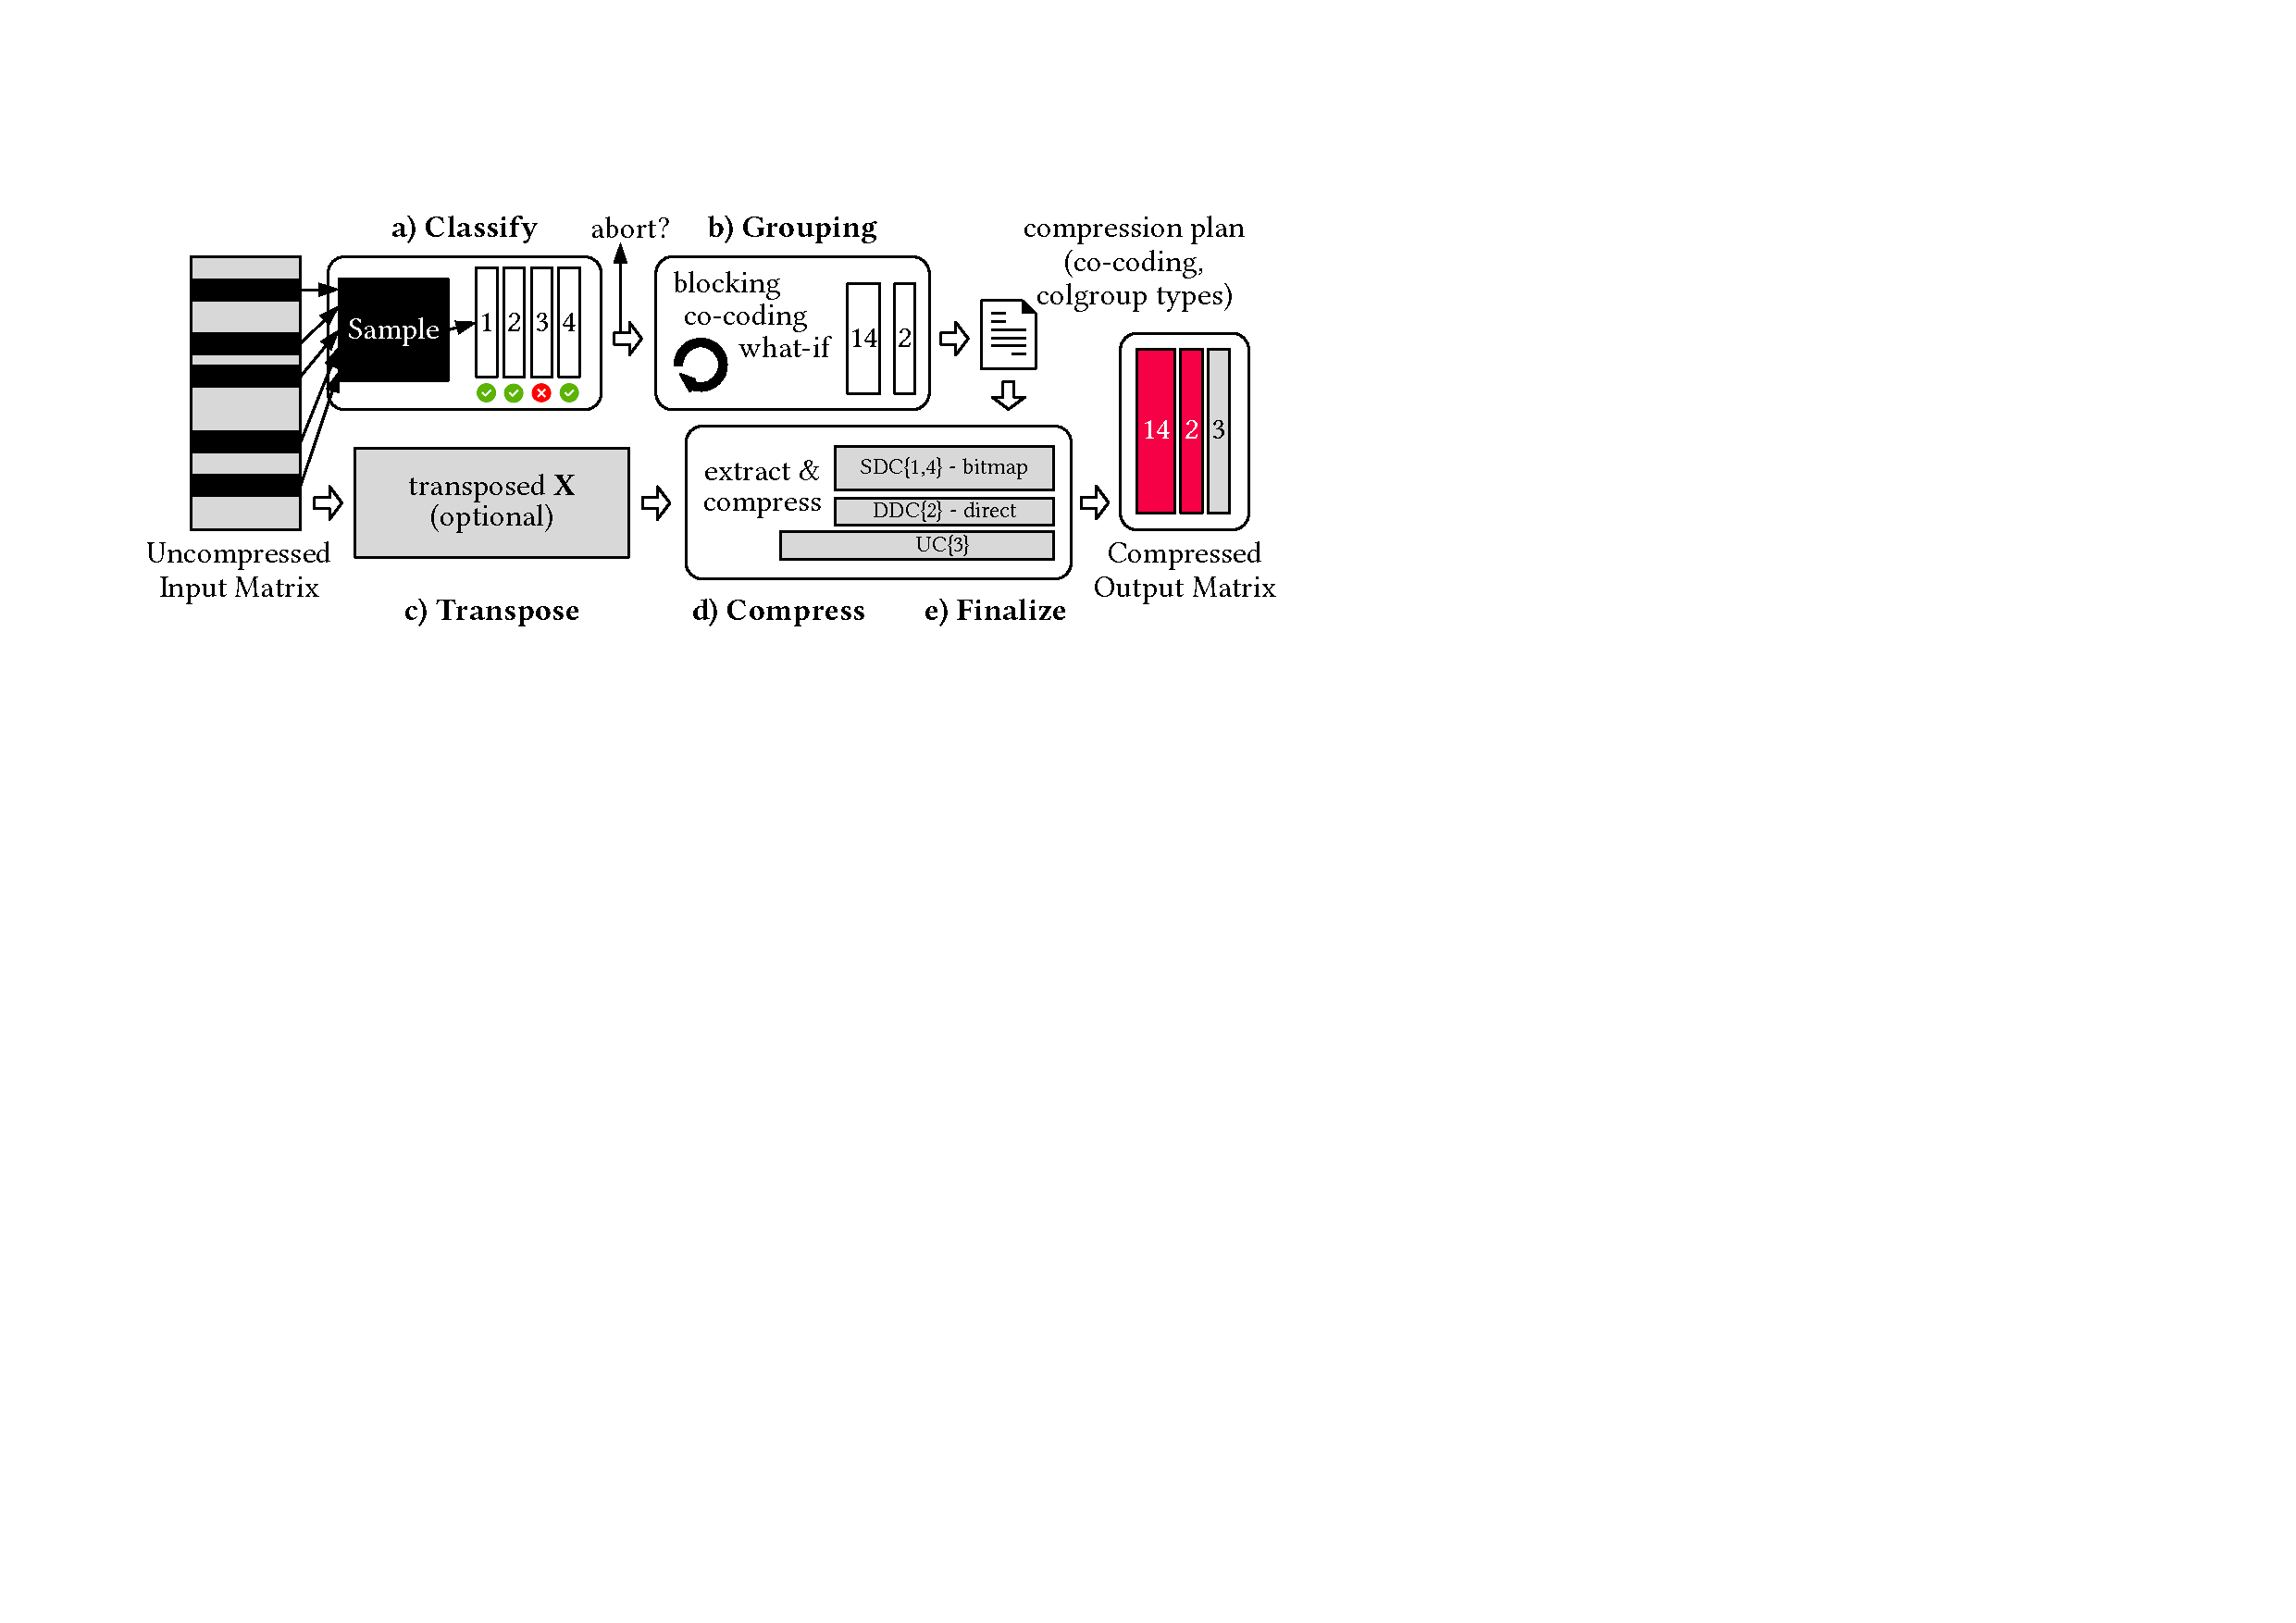
\includegraphics[width=0.8\linewidth ]{fig/fig03}
  \vspace{-0.25cm}
  \caption{\label{fig:phases}Workflow of Compression Phases.}
  \Description{
    A figure showing all the compression phases that are processed.
  }
\end{figure}

\begin{algorithm}[!t]
  \caption{Compression Algorithm}\label{alg:compress}
  \begin{algorithmic}
    \Require{Matrix input $M$}\\
    \Return{$M_c$}
    \State $\textsc{G} \gets \textsc{ExtractIndexStructures}(\textsc{Sample}(M))$
    \State $\textsc{SingleColumInfos} \gets \textsc{Classify(G)}$ \Comment{Abort 1}
    \State $\textsc{Plan} \gets \textsc{Grouping}(\textsc{SingleColumInfos}, G)$ \Comment{Abort 2}
    \State $(M, t) \gets \textsc{TransposeMaybe}(\textsc{Plan}, M)$ \Comment{ t is true if M is transposed}
    \State $M_c \gets \textsc{Finalize}(\textsc{Compress}(\textsc{Plan}, M, t))$ \Comment{Abort 3}
  \end{algorithmic}
\end{algorithm}

\textbf{a) Classify:} For efficient compression planning, we first obtain an index structure (dense or sparse for DDC or SDC) for each column in a sample of the input matrix, as well as counts of non zeros (NNZ) per column in the input matrix. Using the index structure and NNZ count, we compute summary statistics for individual columns (e.g., the frequency of distinct items), estimate the cost of the individual columns, classify columns as compressible or incompressible, and extract empty columns. For classifying a column or list of columns, the same summary statistics are needed, irrespective of optimizing for workload cost or size in memory. Compared to the CLA compression algorithm---where the entire uncompressed matrix was transposed first for efficient extraction in Classify and Compress---we benefit from working only with small index structures until deciding on aborting the compression for non-amenable matrices. Furthermore, we gain more efficient sample extraction, and bounded temporary memory requirements for incompressible matrices.

\begin{algorithm}[!t]
  \caption{Combine Algorithm for Dense Index Structures}\label{alg:combine}
  \begin{algorithmic}
    \Require{Index structures for two groups $I^l, I^r$}\\
    \Return{Combined index structure $I^c$}
    \State $ M \gets I[d_l \cdot d_r]$ , $u \gets 1$ \Comment{Allocate map of possible distinct size}
    \For{ $i \gets 0$ to $n$}
    \State $m \gets I^l_i + I^r_i \cdot d_r$ \Comment{Calculate new unique index}
    \If{$M_m = 0$} \Comment{Non-existing value at the unique index}
    \State $ M_m \gets u\texttt{++} $ \Comment{Assign unique index to next unique value}
    \EndIf
    \State $ I^c_i \gets M_m - 1$ \Comment{Assign output to map value at unique index}
    \EndFor
  \end{algorithmic}
\end{algorithm}


\textbf{b) Grouping:} Column co-coding seeks to find column groups in order to exploit redundancy among correlated columns. \name\ introduces two techniques to improve CLA's co-coding algorithm.
%
First, instead of extracting statistics from the sample when combining columns, we combine the index structures of two already extracted groups from the classification phase or previously combined columns. Algorithm~\ref{alg:combine} combines two dense index structures ($I^r$ and $I^l$) into a combined index structure $I^c$. This algorithm allocates a mapping $M$ that is able to encode all possible unique mappings from combining $I^r$ and $I^l$ by the product of their numbers of distinct items $d_l$ and $d_r$. Further specializations are algorithms for sparse-sparse and sparse-dense combining.
%
Second, we introduce a new co-coding algorithm (see Algorithm~\ref{alg:priorityQueue}) that uses a priority queue $Q$ for sorting columns (or column groups) based on a configurable cost function, and combines groups at the head of the queue. We found that starting with this new co-coding algorithm and switching to a greedy combining approach at a threshold number of remaining groups gives a good balance of compression time and quality. In cases with millions of columns, we do a static partitioning of the columns to available threads and combine columns in a thread-local manner.

\begin{algorithm}[!t]
  \caption{PriorityQueue Co-coding Algorithm}\label{alg:priorityQueue}
  \begin{algorithmic}
    \Require{A queue of all current index structures $Q$}\\
    \Return{A list of index structures $G$}
    \While{$Q.peek \neq NULL$ ,   $I^l \gets Q.poll$} \Comment{Remove cheapest Index}
    \State $I^r \gets Q.peek$                \Comment{Look at next cheapest Index}
    \State $I^c \gets combine(I^l, I^r)$       \Comment{Combine two cheapest}
    \If{$I^c.cost$ < $I^l.cost + I^r.cost$} \Comment{Costs of combined is lower}
    \State $Q.poll$ , $Q.put(I^c)$ \Comment{Remove $I^r$ from queue and add $I^c$}
    \Else
    \State $G.add(I^l)$ \Comment{Add cheapest (already extracted) to output}
    \EndIf
    \EndWhile
  \end{algorithmic}
\end{algorithm}

\textbf{c) Transpose:} The uncompressed input matrix can be transposed (columns in row-major) if the compress phase would benefit from sequential access and amortize such data reorganization. This decision is dependent on the data characteristics (e.g., matrix dimensions, dense or sparse) and the chosen compression plan (e.g., co-coded columns).
% By default, we transpose sparse matrices that have more than 500\text{K} rows or a number of column groups greater than $m/2$ (few co-coded columns).


\textbf{d) Compress:} During compression, we take the input matrix and compression plan (co-coding decisions, and column-group types), and create the compressed column groups. For every group, we first extract its single- or multi-column uncompressed bitmap as a canonical representation of distinct tuples and offset lists per tuple. With these temporary offset lists, we re-evaluate the group types, and finally create the physical encoding of the compressed column groups, which involves various specializations (e.g., delta-encoded offsets) for smaller code words. Once a column group is compressed---and it is beneficial in terms of workload costs---we analyze if we can sparsify its dictionary via a frame-of-reference encoding, and if so apply the transformation. In contrast to CLA, we apply no corrections for estimated compressible but actually incompressible columns because the estimators and co-coding show robust behavior.

\textbf{e) Finalize:} In a last phase, we perform compaction of special groups, and compare costs of the actual compressed representation with the uncompressed costs (and abort if needed). Finally, we cleanup all temporary buffers but keep a soft reference (subject to garbage collection under memory pressure) to the uncompressed block to skip potential decompressions.

\textbf{Parallelization Strategies:} When compressing distributed matrices, blocks are compressed independently in a data-parallel manner with single-threaded compression per block. In contrast, local, in-memory compression utilizes multi-threading with barriers per phase. Classify parallelizes over columns, Grouping over blocks of columns, Compress over column groups and in some cases row partitions, and Transpose uses a multi-threaded cache-conscious uncompressed transpose operation. A more fine-grained parallelization with a task graph \cite{MoritzNWTLLEYPJ18} is interesting future work.
